% ===================================================================
%  Week 11 — Persian lecture notes — Homography & Perspective Warp
% ===================================================================
\documentclass[12pt,a4paper]{article}
% ===================================================================
%  Shared preamble for Persian lecture notes (Image Processing).
%  Compile with XeLaTeX.  Body = Persian (RTL), code/math = LTR.
% ===================================================================

\usepackage{geometry}
\geometry{a4paper,margin=2.4cm}
\usepackage{amsmath,amssymb}
\usepackage{graphicx}
\usepackage{xcolor}
\usepackage{listings}
\usepackage{tcolorbox}
\usepackage{booktabs}
\usepackage{array}
\usepackage{enumitem}
\usepackage{hyperref}
\tcbuselibrary{skins,breakable}

% ---- Persian / RTL --------------------------------------------------
\usepackage{xepersian}
\settextfont{IRNazli}
\setlatintextfont{Latin Modern Roman}
\setdigitfont{IRNazli}
% More generous leading + paragraph spacing (Persian reads better with air).
\linespread{1.5}
\setlength{\parskip}{0.7em}

% ---- Colours --------------------------------------------------------
\definecolor{coursePrimary}{HTML}{1B4965}
\definecolor{courseAccent}{HTML}{E76F51}
\definecolor{courseGood}{HTML}{2A9D8F}
\definecolor{courseBad}{HTML}{C0392B}
\definecolor{courseInfo}{HTML}{2980B9}
\definecolor{codeBg}{HTML}{F5F6FA}
\definecolor{codeKw}{HTML}{8E44AD}
\definecolor{codeStr}{HTML}{2A9D8F}
\definecolor{codeCom}{HTML}{7F8C8D}

\hypersetup{colorlinks=true,linkcolor=courseInfo,urlcolor=courseInfo,citecolor=courseInfo}

% ---- Code listings (Python built in) -------------------------------
\lstdefinestyle{course}{
  backgroundcolor=\color{codeBg},
  basicstyle=\ttfamily\small,
  keywordstyle=\color{codeKw}\bfseries,
  stringstyle=\color{codeStr},
  commentstyle=\color{codeCom}\itshape,
  numberstyle=\tiny\color{codeCom},
  numbers=left, numbersep=7pt,
  showstringspaces=false, breaklines=true,
  tabsize=4, columns=fullflexible, frame=single,
  rulecolor=\color{gray!30}, keepspaces=true, upquote=true, language=Python,
}
\lstset{style=course}
\lstdefinelanguage{bash}{
  keywords={cd,pip,python,venv,source,import}, sensitive=true,
  morecomment=[l]{\#}, morestring=[b]', morestring=[b]",
}
\newenvironment{ltrcode}{\begin{LTR}}{\end{LTR}}

% ---- Callout boxes (Persian titles) --------------------------------
\newtcolorbox{yaddasht}{colback=courseInfo!8,colframe=courseInfo,
  title={\textbf{یادداشت}},boxrule=0.6pt,right=6pt,left=6pt,breakable}
\newtcolorbox{nokte}{colback=courseAccent!10,colframe=courseAccent,
  title={\textbf{نکتهٔ کلیدی}},boxrule=0.6pt,right=6pt,left=6pt,breakable}
\newtcolorbox{hoshdar}{colback=courseBad!8,colframe=courseBad,
  title={\textbf{هشدار / دام}},boxrule=0.6pt,right=6pt,left=6pt,breakable}
\newtcolorbox{riyazi}{colback=coursePrimary!6,colframe=coursePrimary,
  title={\textbf{ریاضیات}},boxrule=0.6pt,right=6pt,left=6pt,breakable}
\newtcolorbox{tamrin}{colback=courseGood!8,colframe=courseGood,
  title={\textbf{تمرین}},boxrule=0.6pt,right=6pt,left=6pt,breakable}

% ---- Header helper --------------------------------------------------
\newcommand{\coursemeta}[2]{%
  \begin{center}
  {\large\textbf{پردازش تصویرِ کاربردی}}\\[2pt]
  {\color{coursePrimary}\rule{\linewidth}{1pt}}\\[4pt]
  {\Large\textbf{#1}}\\[3pt]
  {\small جزوهٔ درس — #2}
  \end{center}\vspace{4pt}
}


\begin{document}
\coursemeta{جلسهٔ ۱۱ — هوموگرافی و تصحیحِ پرسپکتیو (Homography \& Perspective Warp)}{هفتهٔ یازدهم}

\section*{نگاهِ کلی به این جلسه}

تا این هفته یاد گرفتیم مقدارِ پیکسل‌ها را تغییر دهیم (روشنایی، لبه، آستانه) و نقاطِ متناظر را بینِ دو تصویر پیدا کنیم (ویژگی‌ها). این هفته کارِ متفاوتی می‌کنیم: \emph{موقعیتِ} پیکسل‌ها را تغییر می‌دهیم. هدفِ نهایی بسیار ملموس است: کاربر با موبایل از یک کنتور یا سند عکسی \emph{کج و از زاویه} می‌گیرد، و ما می‌خواهیم آن را به یک اسکنِ صاف و روبه‌رو تبدیل کنیم — درست مثلِ یک اسکنرِ واقعی. این کار قلبِ پروژهٔ DocScan است و ابزارِ ریاضیِ آن، \textbf{هوموگرافی} (homography) نام دارد.

\begin{yaddasht}
چرا این مهم است؟ چون در هفته‌های ۱۲ تا ۱۴ می‌خواهیم ارقامِ کنتور را بخوانیم. خواندنِ رقم روی تصویری که صاف و روبه‌رو شده صدها بار آسان‌تر و دقیق‌تر است تا روی عکسی کج و پرسپکتیودار. پس این هفته، «مرحلهٔ آماده‌سازیِ» کلِ سامانه است.
\end{yaddasht}

\subsection*{یک تشبیهِ ساده}

تصور کنید یک تابلوی مستطیلی روی دیوار است و شما از کنار به آن نگاه می‌کنید. در چشمِ شما، تابلو دیگر مستطیل نیست، بلکه یک ذوزنقه است: لبهٔ دور کوچک‌تر از لبهٔ نزدیک دیده می‌شود. مغزِ شما به‌طورِ خودکار می‌داند که تابلو «واقعاً» مستطیل است و آن را تصحیح می‌کند. هوموگرافی دقیقاً همین کارِ مغز را با ریاضی انجام می‌دهد: می‌داند ذوزنقهٔ دیده‌شده باید به مستطیل بازگردد و ماتریسی می‌سازد که این بازگشت را انجام دهد. کلِ این جلسه، آموزشِ همین «تصحیحِ زاویهٔ دید» به کامپیوتر است.

\section{تبدیلِ هندسی چیست؟}

یک \textbf{تبدیلِ هندسی} (geometric transform) تابعی است که به هر پیکسلِ خروجی $(x',y')$ می‌گوید مقدارش را از کدام محلِ تصویرِ ورودی $(x,y)$ بردارد. عملیاتِ قبلی («این پیکسل چه رنگی است؟») را کنار می‌گذاریم و به پرسشِ تازه‌ای پاسخ می‌دهیم: «این نقطه کجا می‌رود؟»

\begin{itemize}
  \item \textbf{انتقال (translation):} جابه‌جاییِ ساده.
  \item \textbf{چرخش و مقیاس (rotation, scale):} چرخاندن و بزرگ/کوچک کردن.
  \item \textbf{برش (shear):} کج‌کردنِ مستطیل به متوازی‌الاضلاع.
  \item \textbf{پرسپکتیو (perspective):} مهم‌ترین برای ما — اثرِ زاویهٔ دوربین.
\end{itemize}

\subsection{سلسله‌مراتبِ تبدیل‌ها}

تبدیل‌های دوبُعدی یک سلسله‌مراتب دارند؛ هر سطح عام‌تر از سطحِ بالای خود است و «درجاتِ آزادیِ» (DoF) بیشتری دارد:

\begin{center}
\begin{tabular}{@{}lll@{}}
\hline
\textbf{تبدیل} & \textbf{چه چیزی را حفظ می‌کند} & \textbf{DoF} \\
\hline
صُلب (چرخش+انتقال) & طول و زاویه & ۳ \\
تشابهی (+مقیاس) & زاویه و نسبت‌ها & ۴ \\
اَفاین (Affine) & موازی‌بودنِ خطوط & ۶ \\
تصویری/هوموگرافی & فقط راستایِ خطوط & ۸ \\
\hline
\end{tabular}
\end{center}

\begin{nokte}
نکتهٔ کلیدی: یک عکس که از زاویه گرفته شده، به عام‌ترین تبدیل نیاز دارد، یعنی \textbf{هوموگرافی}. تبدیل‌های ساده‌تر (مثلِ اَفاین) نمی‌توانند اثرِ پرسپکتیو را مدل کنند.
\end{nokte}

\subsection{اَفاین در برابرِ پرسپکتیو، روی یک شبکه}

بهترین راه برای دیدنِ تفاوت، اعمالِ هر دو تبدیل روی یک شبکهٔ مربعی است:

\begin{center}
  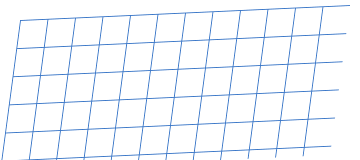
\includegraphics[width=0.44\linewidth]{../assets/grid_affine.png}\hfill
  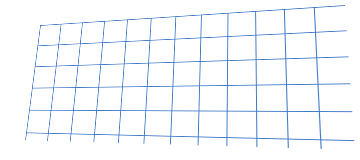
\includegraphics[width=0.44\linewidth]{../assets/grid_perspective.png}\\
  {\small چپ: اَفاین — خطوطِ موازی موازی می‌مانند \quad راست: پرسپکتیو — خطوطِ موازی هم‌گرا می‌شوند}
\end{center}

آن هم‌گراییِ خطوط در تصویرِ راست، همان اثرِ «نقطهٔ گریز» (vanishing point) در دوربینِ واقعی است. فقط هوموگرافی می‌تواند این را مدل کند.

\section{تبدیلِ اَفاین}

تبدیلِ اَفاین ۶ درجهٔ آزادی دارد (یک ماتریسِ $۲\times۳$) و متوازی‌الاضلاع را به متوازی‌الاضلاع می‌نگارد.

\begin{riyazi}
\[
\begin{pmatrix}x'\\y'\end{pmatrix} = A\begin{pmatrix}x\\y\end{pmatrix} + t,\qquad A \in \mathbb{R}^{2\times2},\ t\in\mathbb{R}^2
\]
خطوطِ صاف صاف می‌مانند و خطوطِ موازی موازی می‌مانند. با ۳ نقطهٔ متناظر کاملاً تعیین می‌شود:
\texttt{cv2.getAffineTransform} و سپس \texttt{cv2.warpAffine}.
\end{riyazi}

اَفاین برای چرخش/مقیاس/برش عالی است، اما \emph{نمی‌تواند} صفحه‌ای را که از دوربین دور شده مدل کند — چون در آن حالت خطوطِ موازی باید هم‌گرا شوند و اَفاین این توانایی را ندارد.

\section{هوموگرافی}

\textbf{هوموگرافی} یک ماتریسِ $۳\times۳$ است که دو نمای مختلف از یک سطحِ \emph{تخت} را به هم مربوط می‌کند. ۸ درجهٔ آزادی دارد (درایهٔ نهم فقط یک عاملِ مقیاس است). خطوطِ صاف را به خطوطِ صاف می‌نگارد، اما خطوطِ موازی می‌توانند هم‌گرا شوند — دقیقاً مدلِ عکس‌گرفتن از یک صفحهٔ تخت از هر زاویه.

\begin{riyazi}
با مختصاتِ همگن (homogeneous):
\[
\begin{pmatrix}x'\\y'\\w'\end{pmatrix} = H \begin{pmatrix}x\\y\\1\end{pmatrix},
\qquad H=\begin{pmatrix} h_{11} & h_{12} & h_{13}\\ h_{21} & h_{22} & h_{23}\\ h_{31} & h_{32} & 1 \end{pmatrix}
\]
و سپس پیکسلِ نهایی از تقسیم به دست می‌آید: $\big(x'/w',\ y'/w'\big)$.
\end{riyazi}

\subsection{چرا تقسیم بر $w'$؟ (بخشِ پرسپکتیو)}

آن تقسیمِ نهایی همان چیزی است که اجسامِ دور را کوچک‌تر و خطوطِ موازی را هم‌گرا می‌کند:

\begin{itemize}
  \item در اَفاین، سطرِ آخرِ ماتریس $(0\ 0\ 1)$ است، پس همیشه $w'=1$ و هیچ پرسپکتیوی نداریم.
  \item در هوموگرافی، سطرِ آخر $(h_{31}\ h_{32}\ 1)$ است، پس $w'$ به موقعیتِ نقطه وابسته می‌شود و همین، اثرِ پرسپکتیو را می‌سازد.
\end{itemize}

\begin{nokte}
کلِ تفاوتِ اَفاین و پرسپکتیو در همین «تقسیم بر $w'$» غیرخطی است. اگر این تقسیم نباشد، هوموگرافی به اَفاین فرومی‌کاهد.
\end{nokte}

\subsection{هوموگرافی چطور از نقاط حل می‌شود؟ (DLT)}

شاید بپرسید \texttt{getPerspectiveTransform} پشتِ‌پرده چه می‌کند. الگوریتمِ آن \textbf{DLT} (Direct Linear Transform) نام دارد. برای هر تناظرِ $(x,y)\leftrightarrow(x',y')$ می‌دانیم:
\begin{riyazi}
\[
x' = \frac{h_{11}x + h_{12}y + h_{13}}{h_{31}x + h_{32}y + 1},\qquad
y' = \frac{h_{21}x + h_{22}y + h_{23}}{h_{31}x + h_{32}y + 1}
\]
با ضربِ طرفین در مخرج، این دو رابطه به دو معادلهٔ \emph{خطی} بر حسبِ درایه‌های $H$ تبدیل می‌شوند. ۴ نقطه $\Rightarrow$ ۸ معادلهٔ خطی $\Rightarrow$ ۸ مجهول را یکتا حل می‌کند.
\end{riyazi}

وقتی تعدادِ نقاط بیش از ۴ باشد (مثلِ ده‌ها تطبیق)، دستگاه «فرا‌معین» می‌شود و به‌جای حلِ دقیق، جوابِ کمینه‌مربعات را می‌گیریم (که \texttt{findHomography} با SVD انجام می‌دهد). این هم دقت را بالا می‌برد و هم اثرِ نویز را کم می‌کند.

\begin{nokte}
درسِ مهندسی: تقریباً همیشه بیش از حدِ‌اقلِ داده جمع کنید. ۴ نقطه کافی است اما شکننده؛ ۴۰ نقطه با کمینه‌مربعات، برآوردی پایدار و مقاوم به نویز می‌دهد.
\end{nokte}

\subsection{چند نقطه یک هوموگرافی را تعیین می‌کند؟}

۸ مجهول داریم، پس به ۸ معادله نیاز است. هر تناظرِ نقطه‌ای ۲ معادله می‌دهد (یکی برای $x'$ و یکی برای $y'$)، پس \textbf{۴ تناظرِ نقطه‌ای} کافی است.

\begin{itemize}
  \item برای دقیقاً ۴ نقطه: \texttt{cv2.getPerspectiveTransform(۴ مبدأ, ۴ مقصد)}.
  \item برای ده‌ها تطبیقِ نویزی: \texttt{cv2.findHomography(pts, pts, cv2.RANSAC)}.
\end{itemize}

\begin{yaddasht}
۴ گوشهٔ خوب تمامِ چیزی است که نیاز دارید. در DocScan، این ۴ گوشه همان ۴ گوشهٔ کادرِ سند یا کنتور است — که در هفتهٔ ۹ با \texttt{approxPolyDP} یاد گرفتیم پیدا کنیم.
\end{yaddasht}

\section{تصحیح (Rectification): قلبِ DocScan}

حالا همهٔ قطعات را کنار هم می‌گذاریم. فرآیندِ تبدیلِ عکسِ کج به اسکنِ صاف چهار گام دارد:

\begin{enumerate}
  \item ۴ گوشهٔ سند/کنتور را در عکس پیدا کن (با \texttt{approxPolyDP} از هفتهٔ ۹، یا با تطبیقِ ویژگی).
  \item تصمیم بگیر این گوشه‌ها \emph{کجا باید بروند}: ۴ گوشهٔ یک مستطیلِ تمیز.
  \item هوموگرافیِ «گوشه‌های عکس $\rightarrow$ گوشه‌های مستطیل» را حساب کن.
  \item عکس را با \texttt{warpPerspective} از این هوموگرافی عبور بده: خروجی، اسکنِ صاف و روبه‌روست.
\end{enumerate}

\subsection{گام ۱ و ۲: کنتورِ کج و ۴ گوشه‌اش}

در شکلِ زیر، سمتِ چپ الگوی تمیز (هدف) است و سمتِ راست یک عکسِ کجِ شبیه‌سازی‌شده که ۴ گوشه‌اش با نقاطِ قرمز مشخص شده‌اند:

\begin{center}
  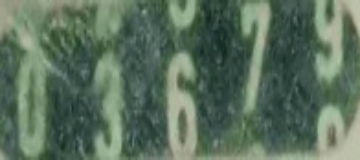
\includegraphics[width=0.44\linewidth]{../assets/original.png}\hfill
  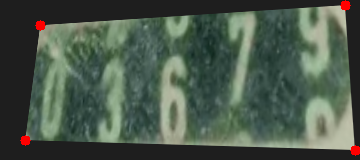
\includegraphics[width=0.44\linewidth]{../assets/tilted.png}\\
  {\small چپ: الگوی تمیز (مقصد) \quad راست: عکسِ کج با ۴ گوشهٔ علامت‌گذاری‌شده}
\end{center}

این ۴ گوشه همان تناظرها هستند: هر نقطهٔ قرمز \emph{کجاست} در برابرِ اینکه \emph{کجا باید باشد}.

\subsection{گام ۳ و ۴: تبدیل به اسکنِ صاف}

با محاسبهٔ هوموگرافی از گوشه‌های عکس به گوشه‌های مستطیل و اعمالِ \texttt{warpPerspective}، عکسِ کج به نمای صاف و روبه‌رو تبدیل می‌شود:

\begin{center}
  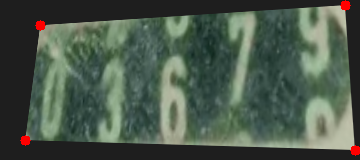
\includegraphics[width=0.44\linewidth]{../assets/tilted.png}\hfill
  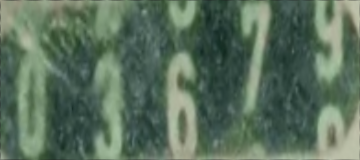
\includegraphics[width=0.44\linewidth]{../assets/recovered.png}\\
  {\small چپ: ورودیِ کج \quad راست: خروجیِ صاف‌شده — ارقام حالا خوانا هستند}
\end{center}

\subsection{یک مثالِ عددی: نگاشتِ یک نقطه}

بیایید ببینیم یک هوموگرافی روی یک نقطه چه می‌کند. فرض کنید
\begin{riyazi}
\[
H = \begin{pmatrix} 1.2 & 0.1 & 5 \\ 0.05 & 1.1 & 8 \\ 0.0005 & 0.0003 & 1 \end{pmatrix},\qquad
\text{نقطهٔ ورودی } (x,y)=(100, 50)
\]
گامِ ۱ — ضربِ ماتریسی:
\begin{align*}
x' &= 1.2(100) + 0.1(50) + 5 = 130 \\
y' &= 0.05(100) + 1.1(50) + 8 = 68 \\
w' &= 0.0005(100) + 0.0003(50) + 1 = 1.065
\end{align*}
گامِ ۲ — تقسیم بر $w'$:
\[
\Big(\tfrac{130}{1.065},\ \tfrac{68}{1.065}\Big) \approx (122.1,\ 63.8)
\]
\end{riyazi}

توجه کنید که اگر سطرِ آخر $(0,0,1)$ بود، $w'=1$ می‌شد و خروجی دقیقاً $(130,68)$ — یعنی یک تبدیلِ اَفاین. آن درایه‌های کوچکِ $0.0005$ و $0.0003$ در سطرِ آخر، همان چیزی هستند که پرسپکتیو را می‌سازند و مقدار را کمی «فشرده» می‌کنند.

\begin{nokte}
همین محاسبهٔ ساده برای \emph{هر} پیکسل تکرار می‌شود. زیباییِ کار این است که یک ماتریسِ کوچکِ $۳\times۳$ کلِ تغییرِ شکلِ پیچیدهٔ پرسپکتیو را کد می‌کند.
\end{nokte}

\subsection{ترتیبِ درستِ گوشه‌ها}

یک نکتهٔ عملیِ حیاتی: \texttt{approxPolyDP} چهار نقطه می‌دهد اما به ترتیبِ \emph{دلخواه}. باید آن‌ها را مرتب کنیم: بالا‌چپ، بالا‌راست، پایین‌راست، پایین‌چپ — وگرنه تصویرِ خروجی می‌چرخد یا آینه می‌شود.

\begin{riyazi}
یک ترفندِ ساده برای مرتب‌کردن: نقطه‌ای که $x{+}y$ کمینه دارد بالا‌چپ است؛ بیشینهٔ $x{+}y$ پایین‌راست؛ کمینهٔ $x{-}y$ بالا‌راست؛ بیشینهٔ $x{-}y$ پایین‌چپ.
\end{riyazi}

\begin{hoshdar}
ترتیبِ غلطِ گوشه‌ها = اسکنِ آینه‌ای یا چرخیده. همیشه گوشه‌ها را با یک قاعدهٔ ثابت مرتب کنید.
\end{hoshdar}

\section{انطباقِ خودکار با RANSAC}

به‌جای انتخابِ دستیِ ۴ گوشه، می‌توانیم از تطبیق‌های ویژگیِ هفتهٔ ۱۰ استفاده کنیم. اما تطبیق‌ها شاملِ موارِد غلط‌اند؛ یک برازشِ ساده با این برون‌داده‌ها خراب می‌شود. راه‌حل، \textbf{RANSAC} است.

\begin{nokte}
RANSAC مخففِ RANdom SAmple Consensus است: تبدیلی را پیدا می‌کند که بیشترین تعدادِ تطبیق‌ها با آن «موافق»‌اند (یعنی درون‌داده یا inlier هستند).
\end{nokte}

\subsection{RANSAC گام‌به‌گام}

\begin{enumerate}
  \item ۴ تناظرِ تصادفی انتخاب کن و یک $H$ کاندید حساب کن.
  \item درون‌داده‌ها را بشمار: تطبیق‌هایی که $H$ نقطه‌شان را با خطای چند پیکسل درست می‌نگارد.
  \item این کار را ده‌ها یا صدها بار تکرار کن و $H$ با بیشترین درون‌داده را نگه دار.
  \item در پایان $H$ را با \emph{همهٔ} درون‌داده‌هایش دوباره برازش کن تا دقیق شود.
\end{enumerate}

\begin{yaddasht}
قدرتِ RANSAC: حتی اگر کسرِ بزرگی از تطبیق‌ها غلط باشند، تا وقتی که ۴ تطبیقِ درست \emph{وجود داشته باشند}، RANSAC آن‌ها را پیدا می‌کند. به همین دلیل استانداردِ طلاییِ برازشِ مقاوم در بینایی ماشین است.
\end{yaddasht}

\subsection{تصحیحِ خودکار روی کنتورِ واقعی}

در پروژهٔ واقعیِ ما، این خط‌لولهٔ کامل روی یک کنتورِ واقعیِ آب اجرا شد: ابتدا ویژگی‌های ORB روی عکسِ کج و الگو استخراج شد، سپس تطبیق داده شد، و در نهایت \texttt{findHomography} با RANSAC تبدیل را برآورد کرد. نتیجه: از \textbf{۶۶ تطبیقِ خوب، ۵۷ درون‌داده} و یک اسکنِ کاملاً صاف — بدونِ هیچ انتخابِ دستیِ گوشه:

\begin{center}
  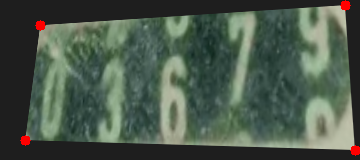
\includegraphics[width=0.44\linewidth]{../assets/tilted.png}\hfill
  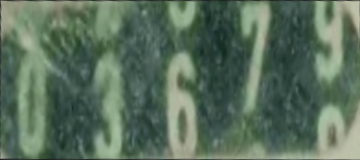
\includegraphics[width=0.44\linewidth]{../assets/auto_rectified.png}\\
  {\small چپ: عکسِ کج \quad راست: تصحیحِ خودکار با ORB + RANSAC (۵۷ درون‌داده از ۶۶ تطبیق)}
\end{center}

\subsection{نگاشتِ مستقیم در برابرِ نگاشتِ معکوس}

یک ظرافتِ پیاده‌سازی: برای پُرکردنِ تصویرِ خروجی، دو راه داریم. در \textbf{نگاشتِ مستقیم} (forward) هر پیکسلِ ورودی را به خروجی می‌فرستیم؛ مشکل این است که برخی پیکسل‌های خروجی خالی می‌مانند و برخی دوبار پُر می‌شوند («سوراخ» و «برخورد»). در \textbf{نگاشتِ معکوس} (inverse) که OpenCV استفاده می‌کند، برای هر پیکسلِ \emph{خروجی} با معکوسِ $H$ برمی‌گردیم و می‌پرسیم مقدارش از کجای ورودی می‌آید — پس هیچ سوراخی نمی‌ماند.

\begin{yaddasht}
به همین دلیل \texttt{warpPerspective} داخلی از $H^{-1}$ استفاده می‌کند و در ترکیب با درون‌یابی، خروجیِ صاف و بدونِ حفره تولید می‌کند. شما فقط $H$ را می‌دهید؛ OpenCV بقیه را انجام می‌دهد.
\end{yaddasht}

\section{ژرف‌نگری}

\subsection{درون‌یابی: پُرکردنِ پیکسل‌های خروجی}

هنگامِ warp، هر پیکسلِ خروجی به یک محلِ \emph{کسری} در تصویرِ ورودی نگاشته می‌شود — جایی بینِ پیکسل‌ها. باید مقدار را «درون‌یابی» (interpolate) کنیم:

\begin{itemize}
  \item \textbf{نزدیک‌ترین همسایه (nearest):} سریع اما پله‌ای/دندانه‌دار.
  \item \textbf{دوخطی (bilinear):} نرم، پیش‌فرضِ خوب برای تصویر (\texttt{INTER\_LINEAR}).
  \item \textbf{دومکعبی (bicubic):} تیزتر اما کندتر.
\end{itemize}

\begin{nokte}
برای تصویرهای معمولی از \texttt{INTER\_LINEAR} استفاده کنید؛ اما برای نقشه‌های برچسب/ماسک (که مقدارشان معنای رده دارد) از \texttt{INTER\_NEAREST}، وگرنه بینِ دو برچسب مقدارِ بی‌معنی ساخته می‌شود.
\end{nokte}

\subsection{فرضِ تخت‌بودن و محدودیت‌هایش}

هوموگرافی فقط برای یک سطحِ \emph{تخت} (یا دوربینی که فقط می‌چرخد) دقیق است. یک صفحهٔ خمیده، یک درپوشِ کنتورِ قوس‌دار، یا اجسامِ سه‌بُعدی این مدل را می‌شکنند.

\begin{hoshdar}
اگر «اسکنِ» شما هنوز در لبه‌ها قوس دارد، سطح تخت نبوده است. یک هوموگرافیِ واحد نمی‌تواند انحنا را تصحیح کند؛ برای صفحهٔ خمیده به «dewarping» (شبکهٔ غیرخطی) نیاز است که فراتر از یک $H$ است.
\end{hoshdar}

\subsection{دو مسیرِ یافتنِ گوشه‌ها: کدام را انتخاب کنیم؟}

در عمل دو راه برای رسیدن به تناظرها داریم و انتخاب به شرایط بستگی دارد:

\begin{itemize}
  \item \textbf{مسیرِ کانتور (هفتهٔ ۹):} لبهٔ بیرونیِ سند را پیدا کن، با \texttt{approxPolyDP} به ۴ گوشه تقریب بزن. سریع و ساده است، اما نیازمندِ آن است که کلِ سند در کادر و لبه‌اش واضح باشد. برای اسکنِ یک برگه روی میزِ تیره عالی است.
  \item \textbf{مسیرِ ویژگی (هفتهٔ ۱۰):} ویژگی‌ها را با یک الگو تطبیق بده و با RANSAC هوموگرافی بگیر. وقتی لبهٔ سند نامشخص است اما بافتِ داخلی غنی است (مثلِ کنتور با ارقام و علائم) بهتر کار می‌کند، و حتی اگر بخشی از سند بیرونِ کادر باشد باز هم جواب می‌دهد.
\end{itemize}

\begin{nokte}
در DocScanِ ما، مسیرِ ویژگی + RANSAC انتخابِ اصلی است، چون کنتور بافتِ داخلیِ غنی دارد و همیشه لبهٔ تمیزی در دسترس نیست. اما داشتنِ هر دو مسیر به‌عنوانِ پشتیبان، سامانه را مقاوم‌تر می‌کند.
\end{nokte}

\subsection{شکست‌های رایج در DocScan و درمانشان}

\begin{itemize}
  \item \textbf{اسکنِ آینه/چرخیده:} گوشه‌ها بد مرتب شده‌اند $\rightarrow$ قاعدهٔ مرتب‌سازیِ $x{\pm}y$ را اعمال کنید.
  \item \textbf{کششِ عجیبِ ارقام:} نسبتِ ابعادِ مستطیلِ مقصد اشتباه است $\rightarrow$ نسبتِ واقعیِ کنتور را اندازه بگیرید.
  \item \textbf{لبه‌ها هنوز قوس دارند:} سطح تخت نبوده (درپوشِ کنتور خمیده) $\rightarrow$ به dewarpingِ غیرخطی نیاز است.
  \item \textbf{هوموگرافیِ بی‌معنی:} تعدادِ درون‌داده‌ها بسیار کم است $\rightarrow$ ویژگیِ بیشتری استخراج کنید یا آستانهٔ RANSAC را تنظیم کنید؛ اگر باز هم کم بود، احتمالاً عکس و الگو واقعاً یکی نیستند.
\end{itemize}

\begin{hoshdar}
همیشه تعدادِ درون‌داده‌های RANSAC را چاپ و بررسی کنید. اگر از یک آستانه (مثلاً ۱۵) کمتر بود، به هوموگرافی اعتماد نکنید و به کاربر پیام دهید که دوباره عکس بگیرد — این یک «نردبانِ اطمینان» در سامانهٔ واقعی است.
\end{hoshdar}

\subsection{کاربردهای دیگرِ هوموگرافی}

\begin{itemize}
  \item \textbf{دوختِ پانوراما:} هر عکس را به یک قابِ مشترک warp کن و ادغام کن.
  \item \textbf{واقعیتِ افزوده:} یک گرافیک را روی یک نشانگرِ تختِ شناسایی‌شده قرار بده.
  \item \textbf{نمای پرنده (bird's-eye):} صحنهٔ جاده/پارکینگ را به نقشهٔ بالا‌به‌پایین تصحیح کن.
  \item \textbf{DocScan:} تصحیح‌گرِ کنتور/پلاکِ ما.
\end{itemize}

\section{کدِ کاملِ تصحیح‌گر}

\begin{ltrcode}
\begin{lstlisting}[language=Python]
import cv2, numpy as np
# corners: 4 page corners found in the photo, ordered TL,TR,BR,BL
W, H = 800, int(800 * 1.414)          # A4-ish output
dst = np.float32([[0,0],[W,0],[W,H],[0,H]])
M = cv2.getPerspectiveTransform(corners, dst)
scan = cv2.warpPerspective(photo, M, (W, H))

# automatic variant (no manual corners): use ORB matches
Hr, mask = cv2.findHomography(pts_photo, pts_template, cv2.RANSAC, 5.0)
scan = cv2.warpPerspective(photo, Hr, (W, H))
print("inliers:", int(mask.sum()))
\end{lstlisting}
\end{ltrcode}

چهار خط، یک عکسِ کج را به یک اسکنِ صاف تبدیل می‌کند — قلبِ DocScan.

\section{تمرینِ کلاسی و پاسخ}

\begin{tamrin}
۱) چرا یک تبدیلِ اَفاین نمی‌تواند صفحه‌ای را که از زاویه عکس گرفته شده صاف کند؟\\
۲) ۴ گوشهٔ سند را در عکس دارید. برای یک اسکنِ به‌نسبتِ A4 با عرضِ ۸۰۰، نقاطِ مقصد چه هستند؟\\
۳) خط‌لولهٔ خودکارِ شما ۲۰۰ تطبیق دارد که ۶۰‌تای آن‌ها غلط‌اند. کدام گام نجاتتان می‌دهد؟
\end{tamrin}

\textbf{پاسخ‌ها:} (۱) اَفاین خطوطِ موازی را موازی نگه می‌دارد، اما عکسِ واقعی آن‌ها را هم‌گرا می‌کند؛ این نیازمندِ «تقسیم بر $w'$» است که فقط هوموگرافی دارد. (۲) نقاطِ مقصد $(0,0),(800,0),(800,1131),(0,1131)$؛ چون نسبتِ A4 حدودِ $۱{:}۱٫۴۱۴$ است، ارتفاع $=800\times1.414\approx1131$. (۳) \textbf{RANSAC} درونِ \texttt{findHomography} — ۶۰ برون‌داده را نادیده می‌گیرد و فقط به درون‌داده‌ها برازش می‌دهد.

\section{چطور کیفیتِ تصحیح را بسنجیم؟}

مثلِ هفتهٔ پیش، به یک معیارِ کمی نیاز داریم تا بدانیم تصحیح خوب بوده یا نه. سه سنجهٔ عملی:

\begin{itemize}
  \item \textbf{تعدادِ درون‌داده‌های RANSAC:} هرچه بیشتر، برازش پایدارتر. زیرِ یک آستانه یعنی بی‌اعتماد.
  \item \textbf{خطای بازتصویر (reprojection error):} پس از یافتنِ $H$، نقاطِ مبدأ را با آن بنگارید و فاصله‌شان با نقاطِ مقصدِ واقعی را بسنجید؛ میانگینِ چند‌پیکسلی خوب است.
  \item \textbf{راست‌بودنِ خطوط:} در اسکنِ نهایی، لبه‌های کادرِ کنتور باید افقی/عمودی باشند؛ اگر کج‌اند، تصحیح ناقص است.
\end{itemize}

\begin{riyazi}
خطای بازتصویر برای یک نقطه: $e_i = \lVert \text{مقصدِ واقعی}_i - H\cdot\text{مبدأ}_i \rVert$. معیارِ کل معمولاً ریشهٔ میانگینِ مربعات (RMSE) روی همهٔ درون‌داده‌هاست. این عدد، «کیفیتِ هندسیِ» اسکن را به‌صورتِ یک کمیتِ قابلِ‌گزارش می‌دهد.
\end{riyazi}

\begin{yaddasht}
در سامانهٔ واقعی، این اعداد را در لاگ ثبت کنید. وقتی نرخِ خطای خواندنِ ارقام (هفته‌های بعد) بالا رفت، اولین جای بررسی این است: آیا تصحیحِ پرسپکتیو ضعیف بوده؟ زنجیرهٔ پردازش را باید بتوان مرحله‌به‌مرحله عیب‌یابی کرد.
\end{yaddasht}

\section{جمع‌بندی}

در این جلسه یاد گرفتیم که تبدیل‌های هندسی موقعیتِ پیکسل‌ها را تغییر می‌دهند و در یک سلسله‌مراتب (صُلب $\to$ اَفاین $\to$ تصویری) قرار می‌گیرند؛ هوموگرافی عام‌ترین تبدیلِ یک سطحِ تخت است و با ۴ تناظر تعیین می‌شود؛ با ترتیب‌دادنِ گوشه‌ها، ساختنِ $H$ و \texttt{warpPerspective} می‌توان یک عکسِ کج را به اسکنِ صاف تبدیل کرد؛ و با \texttt{findHomography} به‌همراهِ RANSAC می‌توان این کار را به‌طورِ خودکار از تطبیق‌های ویژگی انجام داد. این، مرحلهٔ آماده‌سازیِ DocScan است: از هفتهٔ آینده روی همین اسکن‌های صاف، خواندنِ ارقام را با یادگیریِ ماشین و شبکه‌های عصبی آغاز می‌کنیم.

\end{document}
